\documentclass[]{report}
\usepackage{graphicx}

% Title Page
\title{Report on Polarized Light and Its Applications}
\author{Shuoxuan Han}

\begin{document}
\maketitle

\begin{abstract}
	\paragraph{} Polarization is a phenomenon used to describe transverse waves. In a transverse wave, the direction of the oscillation is transverse to the direction of motion of the wave, so the oscillations can have different directions perpendicular to the wave direction\cite{Avadhanulu.(1992)}.
	\paragraph{} The light around us is complicated. It has a bunch of light with various phases and wave lengthes at the same time. What a polarizer can do is to remove some of the light, making many things look a little bit more beautiful.
	\paragraph{} This report introduces the basic principle of polarization and its application as 3D glasses.
\end{abstract}

\section*{Polarized Light}
\subsection*{Definition} The amplitude of natural light vibration is perpendicular to the propagation direction of the light wave. It has not only the uniformity of the time distribution, but also the uniformity of the spatial distribution. If the direction of the light wave vector remains constant, only vibrates in one direction, we call it polarized light. 
\subsection*{Formation}
\paragraph{Reflection and refraction} The first method to generate polarized light is through reflection and refraction. When light hits a surface at an angle called Brewster's angle, the refraction is polarized\cite{David Brewster.(1815)}. \newline\newline
\centerline{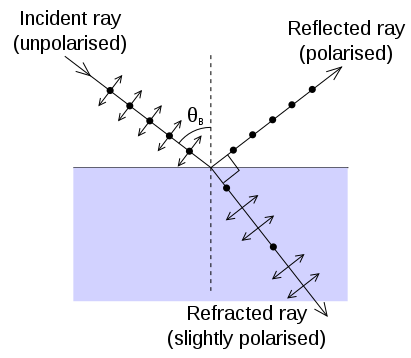
\includegraphics[scale=0.8]{figure3.jpg}}\newline
\centerline{Figure 1}
\paragraph{Polarizer} The other way is using polarizers. It is often called polarizing filters. A polarizer has a lot of long conductive molecules that streches in the same direction like a comb. When light hits the polarizer, it cannot penetrate if it has the polarization in the same direction as the conductive molecules because it will be reflected. Figure 1 helps explain.\newline\newline
\centerline{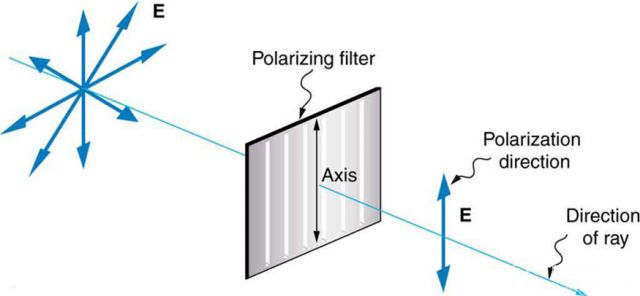
\includegraphics[scale=0.45]{figure1.jpg}}\newline
\centerline{Figure 2}
\newline
\section*{Application}
\paragraph{} One of the most common application of polarizer is 3D glasses. When watching a stereoscopic movie, the audience needs to wear a pair of special glasses, which are perpendicular to each other.\newline\newline
\centerline{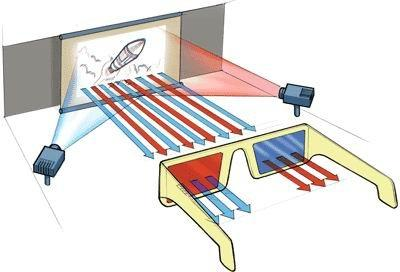
\includegraphics[scale=0.6]{figure4.jpg}}\newline
\centerline{Figure 3}
\paragraph{} Stereoscopic movies are made from two lenses, such as human eyes, which are photographed from two different directions at the same time. When the film is playing, two projectors are used to synchronize the two sets of films captured by two cameras, so that the slightly different two images can overlap on the screen. If you look directly with your eyes, the picture is blurred. To see the stereoscopic film, you have to install a polarizer in front of each camera. The light emitted from two projectors is polarized light after passing through the polarizer. The polarizing directions of the two polarized beams are perpendicular to each other. The two polarized beams are projected onto the screen and reflect to the audience without changing the direction of the polarized light. Putting on the 3D glasses, the audience's each eye sees only the corresponding polarized light image, that is, the left eye can only see the picture left by the left machine, the right eye can only see the picture on the right machine, which will produce stereoscopic feeling. This is the principle of a stereoscopic film and 3D glasses.\newline\newline
\centerline{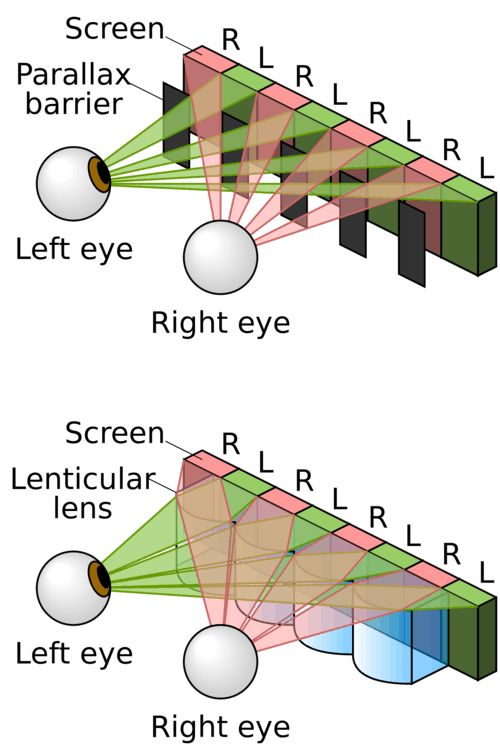
\includegraphics[scale=0.4]{figure2.jpg}}\newline
\centerline{Figure 4}

\begin{thebibliography}{0}
	\bibitem{Avadhanulu.(1992)}
	A Textbook of Engineering Physics. S. Chand Publishing. pp. 198–199. ISBN 8121908175.
	\bibitem{David Brewster.(1815)}
	"On the laws which regulate the polarisation of light by reflection from transparent bodies," Philosophical Transactions of the Royal Society of London, 105: 125-159.	
\end{thebibliography}

\end{document}          
